\chapter{Background}
\section{Gravitational-wave}
\subsection{...}
\section{Sources of Gravitational-wave}
\subsection{...}
\section{Interferometric Gravitational-wave detection} \label{sec:13}

\subsection{Detection Principle}
地上の大型重力波検出器の基本要素はMichelson型レーザー干渉計である。プラスモードの重力波がFig.\ref{img:img}に示すようなMichelson型レーザー干渉計を垂直に通過する場合を考える。

\subsection{Michelson Interferometer}
\begin{figure}[H]
  \begin{center}   
    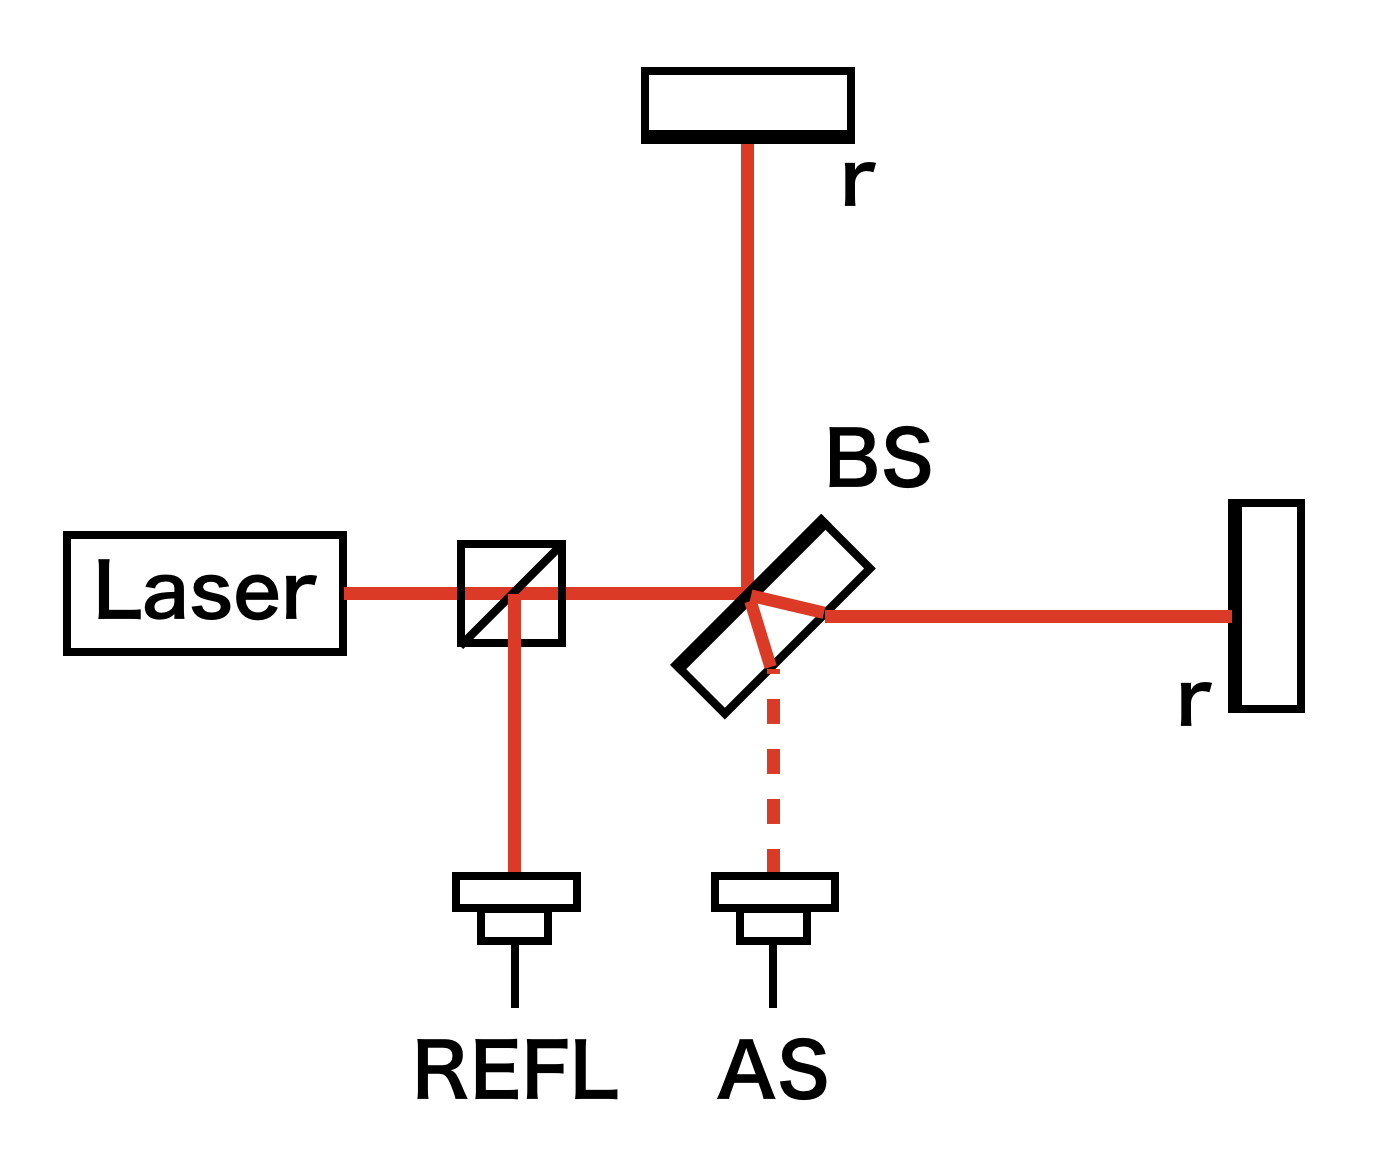
\includegraphics[width=8.0cm]{./img_chap1/img132.png}
    \caption{Michelson Interferometer. }\label{img:img132}
  \end{center}
\end{figure}

Michelson interferometer is a converter from the optical phase difference of two lights to the amplitude modulation of a single light. Consider about the interferometer shown in Fig. \ref{img:img132}. Incident light can be wrtten as,
\begin{eqnarray}
  E_{\mathrm{in}} = E_{0} e^{i\omega{t}},
\end{eqnarray}
where $E_0$ is the amplitude and $\omega_0$ is the angular frequency of the laser field
. Two lights splited by the Beam Spliter (BS) interferer at the Anti-symetric (AS) port and Refrection (REFL) port. The output fieled at the AS port is represented as,
\begin{eqnarray}
  E_{\mathrm{AS}} = -\frac{1}{2}rE_{0} e^{i\left(\omega_{0} t-\phi_{x}\right)}+\frac{1}{2}r E_{0} e^{i\left(\omega_{0} t-\phi_{y}\right)},
\end{eqnarray}
where $r$ denote the amplitude reflectivity of the end mirrors, and $\phi_{x}$ and $\phi_{x}$ are the phase delay due to the light traveling in the $x$ and $y$ arms. This output signal can be represented as a single fieled as,
\begin{eqnarray}\label{eq:eq132}
E_{\mathrm{AS}} = i r E_{0} e^{i\left(\omega_{0} t-\left(\phi_{x}+\phi_{y}\right) / 2\right)} \sin \left(\frac{\phi_{x}-\phi_{y}}{2}\right).
\end{eqnarray}
Wwe find that the amplitude of the output light is a function of the difference between two phases; $\phi_{x}-\phi_{y}$. Furthermore, the power of output light at the AS port is obtained by squaring the Eq.\ref{eq:eq132}, 
\begin{eqnarray}
  P_{\mathrm{AS}} &=\left(r E_{0}\right)^{2}\left[1-\cos \left(\phi_{x}-\phi_{y}\right)\right] 
\end{eqnarray}
Similarly, power of the output light as REFL port is written as,
\begin{eqnarray}
  P_{\mathrm{REFL}} &=\left(r E_{0}\right)^{2}\left[1+\cos \left(\phi_{x}-\phi_{y}\right)\right].
\end{eqnarray}
Therefore, we can measure the optical phase difference as the amplitude changes using a Photo Detector (PD) and detect GWs.

\subsection{Null Measurement}

\subsubsection{Shot Noise}
Shot noise is the optical readout noise associated with the discrete nature of photons and electric charges. 光のパワーは

\subsubsection{Control Noise}
\section{Summary of the Chapter}
